\section{gitc extension}
\label{sec:Extension}
In this section we describe how a cloud9 user can work with our extension and we show how the developing workflow is improved by it.
Further we compare our extension to other tools introduced in section~\needcite{related work}.
Finally we will explain how we intregrated our extension to cloud9 and how we implemented it.

\subsection{Description}
\paragraph{The editor adjustments} of our extension will promt the cloud9 user immediately with visiual feedback of source code changes.
That means while typing in the editor annotations will appear next to the left grutter line as can be seen in figure~\needcite ~\circnum{1}.

The changes show the staged and unstaged changes of the git repository.
We choose to display both type of changes as colored annotations whereas the already staged changes are more transparent. \todo[Vgl. left right anntotation circnum]
The color \textcolor{LimeGreen}{green} is used to visualize added, \textcolor{ProcessBlue}{blue} for changed and \textcolor{Red}{red} for deleted lines.

\begin{figure}
   \centering
   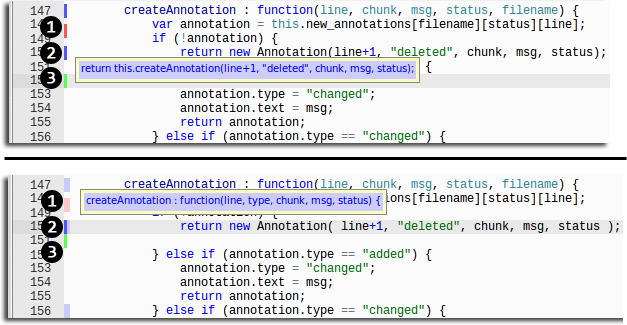
\includegraphics[width=0.9\textwidth]{images/extension_tooltip_comparison.png}
   \caption{Caption}
   \label{fig:editor}
\end{figure}

comparison to earlier editing way, mention history extension (and why we have choosen not to implement stage etc buttons here)

\paragraph{Using our diff view} the cloud9 developer can know ....
By clicking on the pane button \circnum{1} in figure~\needcite or simply using the keyboard shortcut \texttt{strg + g} or \texttt{cmd + g} ....

comparison to earlier diffing, committing

comparison to related work

\subsection{Implementation}
In the following subsections we will describe how we implemented our extension.
First we will have a closer look at how we intregrated our extension to cloud9 and how we execute git commands.
Then we will explain how we implemented the adjustments in the cloud9 editor and the new diff view.

\subsubsection{Integration to cloud9}
%Stephi

\subsubsection{Editor Adjustments}
%Patrick

\subsubsection{Diff View}
%Markus
